% uOttawa (unofficial) Thesis Template for LaTeX 
% Edited by Wail Gueaieb based on Stephen Carr's uWaterloo Template

% The files included in this package are slighly modified by Suruz Miah to adapt partial requirements  in writing project/thesis reports of the Bradley University's Department of Electrical and Computer Engineering.

% DON'T USE THIS TEMPLATE IF YOU DON'T KNOW WHAT YOU'RE DOING!
% Remember, it comes WITH NO WARRANTY!

% Please read the "00readme.txt" file first.
% Here is how to use this template:
%
% DON'T FORGET TO ADD YOUR OWN NAME AND TITLE in the "hyperref" package
% configuration in the "thesis-preample.tex" file. THIS INFORMATION GETS 
% EMBEDDED IN THE PDF FINAL PDF DOCUMENT.
% You can view the information if you view Properties of the PDF document.

% The template is based on the standard "book" document class which provides 
% all necessary sectioning structures and allows multi-part theses.

% DISCLAIMER
% To the best of our knowledge, this template satisfies the current 
% uOttawa thesis requirements.
% However, it is your responsibility to assure that you have met all 
% requirements of the university and your particular department.
% Many thanks to the feedback from many graduates that assisted the 
% development of this template.

% -----------------------------------------------------------------------

% When using pdflatex, by default the output is geared toward generating a PDF 
% version optimized for viewing on an electronic display, including 
% hyperlinks within the PDF.
 
% E.g. to process a thesis based on this template, run:

% (pdf)latex thesisMain	-- first pass of the (pdf)latex processor
% bibtex thesisMain 	-- generates bibliography from .bib data file(s) 
% (pdf)latex thesisMain	-- fixes cross-references, bibliographic references, etc
% (pdf)latex thesisMain	-- fixes cross-references, bibliographic references, etc
% makeindex -s nomentbl.ist -o thesisMain.nls thesisMain.nlo
% (pdf)latex thesisMain	-- fixes cross-references, bibliographic references, etc
% (pdf)latex thesisMain	-- fixes cross-references, bibliographic references, etc



% N.B. The "pdftex" program allows graphics in the following formats to be
% included with the "\includegraphics" command: PNG, PDF, JPEG, TIFF
% Tip 1: Generate your figures and photos in the size you want them to appear
% in your thesis, rather than scaling them with \includegraphics options.
% Tip 2: Any drawings you do should be in scalable vector graphic formats:
% SVG, PNG, WMF, EPS and then converted to PNG or PDF, so they are scalable in
% the final PDF as well.
% Tip 3: Photographs should be cropped and compressed so as not to be too large.

% To create a PDF output that is optimized for double-sided printing: 
%
% 1) comment-out the \documentclass statement in the preamble below, and
% un-comment the second \documentclass line.
%
% 2) change the value assigned below to the boolean variable
% "PrintVersion" from "false" to "true".

% --------------------- Start of Document Preamble -----------------------

% Specify the document class, default style attributes, and page dimensions
% For hyperlinked PDF, suitable for viewing on a computer, use this:
\documentclass[letterpaper,12pt,titlepage,oneside,final]{book}
 
% For PDF, suitable for double-sided printing, change the PrintVersion variable below
% to "true" and use this \documentclass line instead of the one above:
% \documentclass[letterpaper,12pt,titlepage,openright,twoside,final]{book}


% This package allows if-then-else control structures.
\usepackage{ifthen}
\newboolean{PrintVersion}
\setboolean{PrintVersion}{false} 
% \setboolean{PrintVersion}{true} 
% CHANGE THIS VALUE TO "true" as necessary, to improve printed results 
% for hard copies by overriding some options of the hyperref package.


% Load your needed packages and other commands of yours.
% Load your needed packages and other commands of yours here:
%\usepackage{} % ... note that old .sty files can be included here

















%--------------------------------------------------------------------------
% Do NOT edit the rest of the preample UNLESS YOU KNOW WHAT YOU'RE DOING!
%--------------------------------------------------------------------------

\ifthenelse{\boolean{PrintVersion}}{
\usepackage[top=1in,bottom=1in,left=0.75in,right=1.25in]{geometry}   % For twoside document
}{
\usepackage[top=1in,bottom=1in,left=0.75in,right=1.25in]{geometry}   % For oneside document
}

\usepackage{amsmath,amssymb,amstext} % Lots of math symbols and environments
\usepackage{graphicx} % For including graphics 

\usepackage{nomentbl} 
\makenomenclature 

\usepackage{ifpdf}
\usepackage{todonotes}
\newcommand{\href}[1]{#1} % does nothing, but defines the command so the
    % print-optimized version will ignore \href tags (redefined by hyperref pkg).
%\newcommand{\texorpdfstring}[2]{#1} % does nothing, but defines the command
% Anything defined here may be redefined by packages added below...


% Hyperlinks make it very easy to navigate an electronic document.
% In addition, this is where you should specify the thesis title
% and author as they appear in the properties of the PDF document.
% Use the "hyperref" package 
% N.B. HYPERREF MUST BE THE LAST PACKAGE LOADED; ADD ADDITIONAL PKGS ABOVE
\usepackage[\ifpdf pdftex,\fi letterpaper=true,pagebackref=false]{hyperref} % with basic options
		% N.B. pagebackref=true provides links back from the References to the body text. This can cause trouble for printing.
\hypersetup{
    plainpages=false,       % needed if Roman numbers in frontpages
    pdfpagelabels=true,     % adds page number as label in Acrobat's page count
    bookmarks=true,         % show bookmarks bar?
    unicode=false,          % non-Latin characters in Acrobat's bookmarks
    pdftoolbar=true,        % show Acrobat's toolbar?
    pdfmenubar=true,        % show Acrobat's menu?
    pdffitwindow=false,     % window fit to page when opened
    pdfstartview={FitH},    % fits the width of the page to the window
%    pdftitle={uOttawa\ LaTeX\ Thesis\ Template},    % title: CHANGE THIS TEXT!
%    pdfauthor={Author},    % author: CHANGE THIS TEXT! and uncomment this line
%    pdfsubject={Subject},  % subject: CHANGE THIS TEXT! and uncomment this line
%    pdfkeywords={keyword1} {key2} {key3}, % list of keywords, and uncomment this line if desired
    pdfnewwindow=true,      % links in new window
    colorlinks=true,        % false: boxed links; true: colored links
    linkcolor=blue,         % color of internal links
    citecolor=green,        % color of links to bibliography
    filecolor=magenta,      % color of file links
    urlcolor=cyan           % color of external links
}
\ifthenelse{\boolean{PrintVersion}}{   % for improved print quality, change some hyperref options
\hypersetup{	% override some previously defined hyperref options
%    colorlinks,%
    citecolor=black,%
    filecolor=black,%
    linkcolor=black,%
    urlcolor=black}
}{} % end of ifthenelse (no else)

\usepackage{fancyhdr,lastpage} % Change caption style; changes headers and page styles etc.


% This is where thesis margins and spaces are set.
% Setting up the page margins...
% A minimum of 1 inch (72pt) margin at the
% top, bottom, and outside page edges and a 1.125 in. (81pt) gutter
% margin (on binding side). While this is not an issue for electronic
% viewing, a PDF may be printed, and so we have the same page layout for
% both printed and electronic versions, we leave the gutter margin in.
% Set margins:
\setlength{\marginparwidth}{0pt} % width of margin notes
% N.B. If margin notes are used, you must adjust \textwidth, \marginparwidth
% and \marginparsep so that the space left between the margin notes and page
% edge is less than 15 mm (0.6 in.)
\setlength{\marginparsep}{0pt} % width of space between body text and margin notes
\setlength{\evensidemargin}{0.125in} % Adds 1/8 in. to binding side of all 
% even-numbered pages when the "twoside" printing option is selected
\setlength{\oddsidemargin}{0.125in} % Adds 1/8 in. to the left of all pages
% when "oneside" printing is selected, and to the left of all odd-numbered
% pages when "twoside" printing is selected
\setlength{\textwidth}{6.375in} % assuming US letter paper (8.5 in. x 11 in.) and 
% side margins as above
\raggedbottom

% The following statement specifies the amount of space between
% paragraphs. Other reasonable specifications are \bigskipamount and \smallskipamount.
\setlength{\parskip}{\medskipamount}

% The following statement controls the line spacing.  The default
% spacing corresponds to good typographic conventions and only slight
% changes (e.g., perhaps "1.2"), if any, should be made.
\renewcommand{\baselinestretch}{1} % this is the default line space setting

% By default, each chapter will start on a recto (right-hand side)
% page.  We also force each section of the front pages to start on 
% a recto page by inserting \cleardoublepage commands.
% In many cases, this will require that the verso page be
% blank and, while it should be counted, a page number should not be
% printed.  The following statements ensure a page number is not
% printed on an otherwise blank verso page.
\let\origdoublepage\cleardoublepage
\newcommand{\clearemptydoublepage}{%
  \clearpage{\pagestyle{empty}\origdoublepage}}
\let\cleardoublepage\clearemptydoublepage



\fancypagestyle{myFancy}{%
  \fancyhf{}% Clear header and footer
  \fancyhead[LE,RO]{\bfseries\nouppercase{\rightmark}}
  \fancyhead[LO,RE]{\bfseries\nouppercase{\leftmark}}
  \fancyfoot[R]{Page \thepage\ of \pageref{LastPage}}% Custom footer
  \fancyfoot[L]{S.~Miah (\nameOfUniversity)}% Custom footer
  \renewcommand{\headrulewidth}{0.4pt}% Line at the header visible
  \renewcommand{\footrulewidth}{0.1pt}% Line at the footer visible
}


%======================================================================
%   L O G I C A L    D O C U M E N T -- the content of your thesis
%======================================================================
\begin{document}

% For a large document, it is a good idea to divide your thesis
% into several files, each one containing one chapter.
% To illustrate this idea, the "front pages" (i.e., title page,
% declaration, borrowers' page, abstract, acknowledgements,
% dedication, table of contents, list of tables, list of figures,
% nomenclature).
%----------------------------------------------------------------------
% FRONT MATERIAL
%----------------------------------------------------------------------
%
% C O V E R  P A G E
% ------------------
\newcommand{\thesisauthor}{Reece Bachman and Jordan Ingram and Robert O'Malley}
\newcommand{\advisor}{Dr. Suruz Miah}
\newcommand{\thesistitlecoverpage}{%
Building Energy Managment Internet of Things 
}
%\newcommand{\degree}{Ph.D.} % possible values are:
                            % M.A. / M.A.Sc. / M.Sc. / MCS / Ph.D.
\newcommand{\nameofprogram}{Electrical and Computer Engineering Department}
\newcommand{\academicunit}{Caterpillar College of Engineering and Technology}
%\newcommand{\faculty}{Faculty of Engineering}
\newcommand{\nameOfUniversity}{Bradley University}
\newcommand{\graduationyear}{2019}
%
% T I T L E   P A G E
% -------------------
% Last updated May 24, 2011, by Stephen Carr, IST-Client Services
% The title page is counted as page `i' but we need to suppress the
% page number.  We also don't want any headers or footers.
\pagestyle{empty}
\pagenumbering{roman}

% The contents of the title page are specified in the "titlepage"
% environment.
\begin{titlepage}
        \begin{center}
        \vspace*{1.0cm}

        \Huge
        {\bf \thesistitlecoverpage }

        \vspace*{1.0cm}

        \normalsize
        by \\

        \vspace*{1.0cm}

        \Large
        \thesisauthor\\
        Advisor:~\advisor\\

        \vspace*{3.0cm}

        % \normalsize
        % Thesis submitted to the\\
        % Faculty of Graduate and Postdoctoral Studies\\
        % In partial fulfillment of the requirements\\
        % For the \degree~degree in\\
        % \nameofprogram\\

        \vspace*{2.0cm}

        \nameofprogram\\
        \academicunit\\
        %\faculty\\
        \nameOfUniversity\\

        \vspace*{4.0cm}

        \copyright~\thesisauthor, Peoria, Illinois, \graduationyear\\
        \end{center}
\end{titlepage}

% The rest of the front pages should contain no headers and be numbered using Roman numerals starting with `ii'
% PRELIMINARY PAGES

\pagestyle{plain}
\setcounter{page}{2}

\cleardoublepage % Ends the current page and causes all figures and tables that have so far appeared in the input to be printed.
% In a two-sided printing style, it also makes the next page a right-hand (odd-numbered) page, producing a blank page if necessary.



%%% Local Variables:
%%% mode: latex
%%% TeX-master: "../thesisMain"
%%% End:




%
% R E S T  O F  F R O N T  P A G E S
% ----------------------------------
% % D E C L A R A T I O N   P A G E
% -------------------------------
  % This page is not needed for a uOttawa thesis. Don't include it.
  % It is designed for an electronic thesis.
  \noindent
I hereby declare that I am the sole author of this thesis. This is a true copy of the thesis, including any required final revisions, as accepted by my examiners.

  \bigskip
  
  \noindent
I understand that my thesis may be made electronically available to the public.

\cleardoublepage
%\newpage
 %This is not needed in a uOttawa thesis.
%
% Edit the following 3 files with your abstract, acknowledgements, 
% and dedication.
% A B S T R A C T
% ---------------

\begin{center}\textbf{Abstract}\end{center}

This paper presents a method for controlling multiple Internet of Things (IoT) devices. This work uses an open source software from Virginia Tech called Building Energy Management Open Source Software (BEMOSS) to connect multiple IoT devices to one server. This server is run on a linux laptop and manage a variety of IoT devices. This papers work allows the use of BEMOSS on a Raspberry Pi, a cheap commercially available microcontroller, to run commands through BEMOSS. Currently BEMOSS supports a number of commercial IoT devices and in this work, a new device, a DC motor, has been implemented to be run on BEMOSS. Lastly a heating, ventilating, and air conditioning (HVAC) control algorithm has been implemented to be later introduced onto BEMOSS. 
\cleardoublepage
%\newpage


%%% Local Variables:
%%% mode: latex
%%% TeX-master: "../finalReportMainV1"
%%% End:

% A C K N O W L E D G E M E N T S
% -------------------------------

\begin{center}\textbf{Acknowledgements}\end{center}

I would like to thank all the little people who made this possible.


\cleardoublepage
%\newpage



%%% Local Variables:
%%% mode: latex
%%% TeX-master: "../finalReportMainV1"
%%% End:

% D E D I C A T I O N
% -------------------

\begin{center}\textbf{Dedication}\end{center}

This is dedicated to the one I love.


\cleardoublepage
%\newpage


%%% Local Variables:
%%% mode: latex
%%% TeX-master: "../finalReportMainV1"
%%% End:

%
%
% No need to edit this file.
% T A B L E   O F   C O N T E N T S
% ---------------------------------
\renewcommand\contentsname{Table of Contents}
\tableofcontents
\cleardoublepage
\phantomsection
%\newpage

% L I S T   O F   T A B L E S
% ---------------------------
\addcontentsline{toc}{chapter}{List of Tables}
\listoftables
\cleardoublepage
\phantomsection		% allows hyperref to link to the correct page
%\newpage

% L I S T   O F   F I G U R E S
% -----------------------------
\addcontentsline{toc}{chapter}{List of Figures}
\listoffigures
\cleardoublepage
\phantomsection		% allows hyperref to link to the correct page
%\newpage


%
% No need to edit this file. But you may want to comment the whole line if you
% don't have or want a Nomenclature section.
% L I S T   O F   S Y M B O L S
% -----------------------------
% To include a Nomenclature section
\addcontentsline{toc}{chapter}{\textbf{Nomenclature}}

\renewcommand{\nomname}{Nomenclature}
\renewcommand{\nomAname}{\textbf{\large Abbreviations}}
\renewcommand{\nomGname}{\textbf{\large Mathematical Symbols}}
\renewcommand{\nomXname}{\textbf{\large Superscripts}}
\renewcommand{\nomZname}{\textbf{\large Subscripts}}

\printnomenclature
\cleardoublepage
\phantomsection % allows hyperref to link to the correct page
% \newpage






%%% Local Variables: 
%%% mode: latex
%%% TeX-master: "../uottawa-thesis"
%%% End:   


% Change page numbering back to Arabic numerals
\pagenumbering{arabic}



%

% Redefine the plain page style
\fancypagestyle{plain}{%
  \fancyhf{}%
  \fancyfoot[R]{Page \thepage\ of \pageref{LastPage}}%
  \fancyfoot[L]{S.~Miah (\nameOfUniversity)}%  
  \renewcommand{\headrulewidth}{0pt}% Line at the header invisible
  \renewcommand{\footrulewidth}{0.1pt}% Line at the footer visible
}

\pagestyle{myFancy}


%----------------------------------------------------------------------
% MAIN BODY
%---------------------------------------------------------------------- 
% Chapters 
% Include your "sub" source files here (must have extension .tex)
%======================================================================
\chapter{Introduction}
%======================================================================
As smart power grids become more prevalent and data on smart building energy usage becomes more available, the opportunity for energy efficiency increases drastically. Data collected from smart buildings allows a neural network to control the workings of a building in an efficient manner. We propose to expand on the loads that can be controlled through BEMOSS by enabling control of a DC motor. Building energy management open source software (BEMOSS) is an internet of things (IoT) software that was developed at Virginia Tech. This proposed control of a DC motor through an IoT software presents the opportunity to close blinds, open barriers, and move objects throughout the building. The ability to open and close blinds building wide permits the ability to regulate the interior temperature of a building with a considerably lower power consumption. For instance, closing blinds during a hot day will naturally cool a room while opening blinds during a cold day will naturally heat the room. This added ability to control the interior environment will reduce the energy consumed by a heating ventilation air conditioning (HVAC) system. 
\todo[inline]{Add networking info and controlling python scripting on BEMOSS}
%----------------------------------------------------------------------
\section{Background Study}
%----------------------------------------------------------------------
Authors in~\cite{Han2014} proposed a energy management system based around Zigbees and PLCs. Han's system would place a energy measurement and communication unit in each outlet and light in the consumer's home. The energy usage will be measured and the data collected will be sent to a home server run on a Zigbee. These Zigbees will analyze the data and give feedback to the user on how to better manage their energy usage. Renewable energy will be connected to a PLC to allow the use of renewables as they need to converted to AC. The home server on the Zigbee will predict the amount of energy that will be obtained by renewables by accessing weather data and automatically adjust the user's device schedule.

In~\cite{Collotta2015} the authors once again proposed sensors in all outlets and lights to measure the energy usage in homes. Renewable energy sources, like solar panels and wind energy, are connected to an inverter and battery system, to allow the storage of excess power. Collotta connects the internet of things devices using Bluetooth rather than WiFi, due to the lower power consumption. The system checks the current time and cross checks it with the peak time for energy consumption by the user's energy provider. If it is during peak times, the system checks the battery system for excess stored energy. When the user is trying to use energy during a peak time and without a battery charge the system warns the user, but allows the user to ignore these warnings.

In~\cite{Mantovani2014} the energy system uses two model predictive controllers (MPC), one for the building's HVAC system and one for the system's battery power flow. The building's energy management system predicts the temperature of each room separately using sensors and a Kalman filter for robustness. The battery system put in place by Mantovani can run on two modes, one to minimize energy cost and another to minimize power flow. The building is also c-onnected to wind turbines and photo-voltaic cells and predicts the energy produced using a simplified model.

The authors in~\cite{Hannan2018} propose a Internet of Energy network rather than an IoT network. An IoE combines IoT and smart grid technology using four key components: Energy Router, Storage System, renewable sources, and plug-and-play appliances. The IoE allows for an easier way to produce a net zero energy building, that produces as much or more energy than it consumes. The energy router consists of a solid-state-transformer, grid control, and communication meant for data management. The storage system like batteries, reduce the stress on the power grid and lower voltage fluctuation. Renewable sources reduce carbon emmisions, however they reduce harmonics that need to be handled with additional hardware. Lastly the plug-and-play appliances are the devices that the end-user uses in a home.

In~\cite{Pan2015} the system heavily interfaces with the users' smartphones as a way to monitor the building occupants. Since smartphones almost all have a way to track GPS, the system tracks the users' location and send it to the building's server. The building's server is broken up into a number of subservers to handle an individual room's needs. By tracking location the building can do such things like pre-heating or pre-cooling a room before the user is even in the building. All the subservers are connected to the main server which is connected to cloud storage which is used for hosting the large amount of data and handling the intense computations.


\section{Project Statement}
Our project had three main goals. The first goal was to implement a new device not currently supported by BEMOSS on BEMOSS. The second goal was to run BEMOSS on a single board computer, such as a raspberry pi. The last goal is to develop a control algorithm to reduce energy cost and implement the algorithm on BEMOSS.

\section{Report Structure}

%%% Local Variables:
%%% mode: latex
%%% TeX-master: "../finalReportMainV1"
%%% End:

% Some LaTeX commands I define for my own nomenclature.
% If you have to, it's better to change nomenclature once here than in a 
% million places throughout your thesis!
\newcommand{\package}[1]{\textbf{#1}} % package names in bold text
\newcommand{\cmmd}[1]{\textbackslash\texttt{#1}} % command name in tt font 


%======================================================================
\chapter{Observations}
%======================================================================

This would be a good place for some figures and tables.

Some notes on figures and photographs\ldots

\begin{itemize}
\item A well-prepared PDF should be 
  \begin{enumerate}
    \item Of reasonable size, {\it i.e.} photos cropped and compressed.
    \item Scalable, to allow enlargment of text and drawings. 
  \end{enumerate} 
\item Photos must be bit maps, and so are not scaleable by definition. TIFF and
BMP are uncompressed formats, while JPEG is compressed. Most photos can be
compressed without losing their illustrative value.
\item Drawings that you make should be scalable vector graphics, \emph{not} 
bit maps. Some scalable vector file formats are: EPS, SVG, PNG, WMF. These can
all be converted into PNG or PDF, that pdflatex recognizes. Your drawing 
package probably can export to one of these formats directly. Otherwise, a 
common procedure is to print-to-file through a Postscript printer driver to 
create a PS file, then convert that to EPS (encapsulated PS, which has a 
bounding box to describe its exact size rather than a whole page). 
Programs such as GSView (a Ghostscript GUI) can create both EPS and PDF from PS files.
Appendix~\ref{ch:Appendix-Matlab} shows how to generate properly sized Matlab plots and save them as PDF.
\item It's important to crop your photos and draw your figures to the size that
you want to appear in your thesis. Scaling photos with the 
includegraphics command will cause loss of resolution. And scaling down 
drawings may cause any text annotations to become too small.
\end{itemize}
 
For more information on \LaTeX\, see the uWaterloo Skills for the Academic Workplace 
course notes at \href{http://saw.uwaterloo.ca/latex}{saw.uwaterloo.ca/latex}. 
\footnote{
Note that while it is possible to include hyperlinks to external documents,
it is not wise to do so, since anything you can't control may change over time. 
It \emph{would} be appropriate and necessary to provide external links to 
additional resources for a multimedia ``enhanced'' thesis. 
But also note that if the \package{hyperref} package is not included, 
as for the print-optimized option in this thesis template, any \cmmd{href} 
commands in your logical document are no longer defined.
A work-around employed by this thesis template is to define a dummy \cmmd{href} 
command (which does nothing) in the preamble of the document, 
before the \package{hyperref} package is included. 
The dummy definition is then redifined by the
\package{hyperref} package when it is included.
}

The classic book by Leslie Lamport~\cite{lamport.book}, author of \LaTeX , is worth a look too, and the many available add-on packages are described by 
Goossens \textit{et~al.}~\cite{goossens.book}. Some on-line documentation is linked
to from \href{http://saw.uwaterloo.ca/latex}{saw.uwaterloo.ca/latex}. 



Here is an example of how to include figures in \LaTeX. 
Figure~\ref{fig.beam} shows a cantilever beam of circular cross-section
subjected to a point load and a uniformly distributed load, both of which are uncertain. Note that it is better not to include the extension of the figure's source file.

\begin{figure}[!htbp]
 \begin{center}
  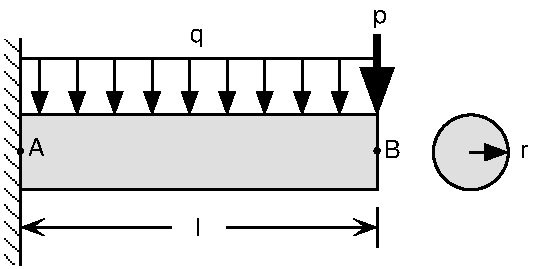
\includegraphics[clip=true]{figs/ipe/beam}
 \end{center}
\caption{Cantilever Beam}
\label{fig.beam}
\end{figure}



%----------------------------------------------------------------------
\section{Adding Nomenclature}
%----------------------------------------------------------------------

The following example is part of the ``nomentbl'' package. Refer to the package's documentation for more details.

\bigskip

\noindent
Let's start with equations to show how to use greek and mathematical symbols within Nomenclature.

Here is an equation
%
\begin{equation}\label{eq:heatflux}
  \dot{Q} = k \cdot A \cdot \Delta T
\end{equation}%
%
%% Greek and math symbols
% \nomenclature[gQ]{$\dot{Q}$}{heat flux}{W}{}%
% \nomenclature[gk]{$k$}{overall heat transfer coefficient}{$\frac{\mathrm{W}}{\mathrm{m}^2\mathrm{K}}$}{see eq.~(\ref{eq:ohtc})}%
% \nomenclature[gA]{$A$}{area}{m$^2$}{$L^2$}%
% \nomenclature[gL]{$L$}{length}{m}{SI base quantity}%
% \nomenclature[gT]{$T$}{temperature}{K}{SI base quantity}%
% \nomenclature[gT]{$\Delta T$}{temperature difference}{K}{SI base quantity}%

% Here is another one
% %
% \begin{equation}\label{eq:ohtc}
%   \frac{1}{k} = \left[\frac{1}{\alpha _{\mathrm{i}}\,r_{\mathrm{i}}} +
%     \sum^n_{j=1}\frac{1}{\lambda _j}\,
%     \ln \frac{r_{\mathrm{a},j}}{r_{\mathrm{i},j}} +
%     \frac{1}{\alpha _{\mathrm{a}}\,
%       r_{\mathrm{a}}}\right] \cdot r_{\mathrm{reference}}
% \end{equation}%
% %
% %% Greek and math symbols
% \nomenclature[ga]{$\alpha$}{convection heat transfer coefficient}{$\frac{\mathrm{W}}{\mathrm{m}^2\mathrm{K}}$}{}%
% \nomenclature[gl]{$\lambda$}{thermal conductivity}{$\frac{\mathrm{W}}{\mathrm{m K}}$}{}%
%
%% Subscripts
% \nomenclature[za]{a}{out}{}{}%
% \nomenclature[zi]{i}{in}{}{}%
% \nomenclature[zj]{$j$}{running parameter}{}{}% 
% \nomenclature[zn]{$n$}{number of walls}{}{}%


% \bigskip

% \noindent
% The following example is to show how to use abbreviations within the Nomenclature.\\
% EECS is a school at the UO.
% %% Abbreviations
% \nomenclature[a]{EECS}{Electrical Engineering and Computer Science}{}{}%
% \nomenclature[a]{UO}{University of Ottawa}{}{}%



\bigskip

\noindent
Don't forget to run:
\begin{verbatim}
makeindex -s nomentbl.ist -o uottawa-thesis.nls uottawa-thesis.nlo
\end{verbatim}



%%% Local Variables:
%%% mode: latex
%%% TeX-master: "../finalReportMainV1"
%%% End:

%======================================================================
\chapter{Control Algorithm}
%======================================================================
To start the group wanted to create an algorithm that would monitor all devices on BEMOSS and use machine learning to optimize the consumer's behavior. To begin however we developed models for an HVAC system that could currently be controlled on BEMOSS but has no built in energy management support and a model of a motor that we developed to be controlled on BEMOSS. 
%----------------------------------------------------------------------
\section{System Modeling}
%----------------------------------------------------------------------
To develop our models we used Matlab and Simulink and created block diagram models for a HVAC system as well as a motor controlled using a PWM signal and H-bridge. To create realistic models we used a Simulink library, Simscape, that has built in electromechanical blocks that we can adjust the parameters of to better model our real world system.

\subsection{Motor}
The model of the motor was based on the initial design constraints of our hardware. 
\begin{figure}
    \centering
    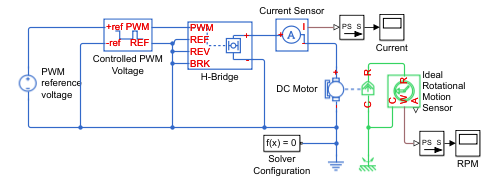
\includegraphics{figs/img/motorModelWithHBridge.png}
    \caption{Motor Model in Simulink}
    \label{fig:my_label}
\end{figure}
As can be noted the model is controlled witha  PWM signal and H-bridge that can be used to run the motor in clockwise and counterclockwise directions. A current sensor is used to read the current output so that the power calculation can be done later in the model. A rotational sensor reads the rotation of the motor in rotations per minute. The DC motor is based on the Pittman 24V DC motor we are currently controlling through BEMOSS in the lab. To do this a DC motor block from simscape is used and the specifications are defined as they appear in the Pittman datasheet. This allows an accurate reading, however it should be noted that the blocks used in Simulink are ideal blocks with no losses to friction or transmission losses. 
\subsection{HVAC Model}
\begin{figure}
    \centering
    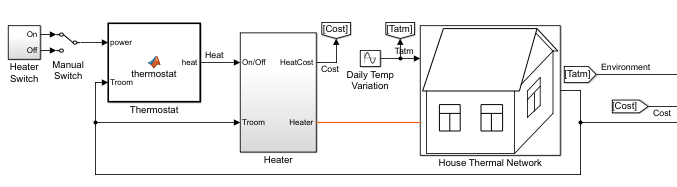
\includegraphics[scale = 0.85]{figs/img/houseModel.PNG}
    \caption{HVAC House Model}
    \label{fig:my_label}
\end{figure}
In this HVAC House Model in Figure 3.2, the thermal properties of a one room home is modeled. An on-off heating control is used to control the temperature of the house. A thermostat block is used to determine if the current temperature in the house model is below the reference signal and using this basic check switches the heating system on or off. The house model itself exchanges heat between three components: air to window, air to wall, and air to roof. This is a simple modeling that is used to show the typical behavior of a house, even if the house itself is not a real world object. The outside temperature is a fluctuating sine wave to determine if the simple on off control will handle changes in temperature. 

\subsection{State-Space Representation of HVAC System}
To better design a more realistic model the team looked at the works of \cite{Kang2014}. The design put forth by the team in \cite{Kang2014} is designed using a State-Space Representation. The typical control problem is defined as 
\begin{equation}
    \Dot{x} = Ax+Bu
\end{equation}
The system used in \cite{Kang2014} is a conventional HVAC system used in many buildings that controls temperature and humidity. In addition the system also measures and controls $CO_2$. 
\newline
To begin a conventional HVAC system that controls only temperature and humidity will be defined and later in the report, built upon to include $CO_2$ monitoring. 

\section{Control of HVAC Model}

%%% Local Variables:
%%% mode: latex
%%% TeX-master: "../finalReportMainV1"
%%% End:


\chapter{Implementing BEMOSS}
Our first task wen learning about 

\section{Deploying BEMOSS}
%Our first task when given this assignment was to download and install BEMOSS onto our laptop so that we could get familiar with the software. Considering BEMOSS only runs on Ubuntu Linux 16.04, we installed VirtualBox version 5.2.14 to try and run Linux.
We were able to run Linux fine but had issues with ssh
\input{parts/50-Hardware.tex}

% %----------------------------------------------------------------------
% % APPENDICES
% %---------------------------------------------------------------------- 
% \appendix
% % Designate with \appendix declaration which just changes numbering style 
% % from here on
% % Add a title page before the appendices and a line in the Table of Contents
% \chapter*{APPENDICES}
% \addcontentsline{toc}{chapter}{APPENDICES} 
% %
% % An appendix
%======================================================================
\chapter{Sources of Information and Help}
\label{ch:Appendix-Sources-of-Info}
%======================================================================
The best source of information about \LaTeX\ is the two books mentioned in this course \cite{lamport.book,goossens.book}.
Another excellent resource is the UseNet newsgroup \verb=comp.text.tex=.
A frequently-asked-questions (FAQ) list is also maintained by this news group.
You might also search the World Wide Web for ``LaTeX'' for other sources of help.


%%% Local Variables:
%%% mode: latex
%%% TeX-master: "../finalReportMainV1"
%%% End:
 %"Sources of Information and Help"
% % An appendix
%======================================================================
\chapter[PDF Plots From Matlab]{Matlab Code for Making a PDF Plot}
\label{ch:Appendix-Matlab} 
%======================================================================
\section{Using the GUI}
Properties of Matab plots can be adjusted from the plot window via a graphical interface. Under the Desktop menu in the Figure window, select the Property Editor. You may also want to check the Plot Browser and Figure Palette for more tools. To adjust properties of the axes, look under the Edit menu and select Axes Properties.

To set the figure size and to save as PDF or other file formats, click the Export Setup button in the figure Property Editor.

\section{From the Command Line} 
All figure properties can also be manipulated from the command line. Here's an example: 
\begin{verbatim}
x=[0:0.1:pi];
hold on % Plot multiple traces on one figure
plot(x,sin(x))
plot(x,cos(x),'--r')
plot(x,tan(x),'.-g')
title('Some Trig Functions Over 0 to \pi') % Note LaTeX markup!
legend('{\it sin}(x)','{\it cos}(x)','{\it tan}(x)')
hold off
set(gca,'Ylim',[-3 3]) % Adjust Y limits of "current axes"
set(gcf,'Units','inches') % Set figure size units of "current figure"
set(gcf,'Position',[0,0,6,4]) % Set figure width (6 in.) and height (4 in.)
cd n:\thesis\plots % Select where to save
print -dpdf plot.pdf % Save as PDF
\end{verbatim} 


%%% Local Variables:
%%% mode: latex
%%% TeX-master: "../finalReportMainV1"
%%% End:
 %"Matlab Code for Making a PDF Plot"

% %----------------------------------------------------------------------
% % END MATERIAL
% %----------------------------------------------------------------------

% % B I B L I O G R A P H Y
% % -----------------------
% %
% % The following statement selects the style to use for references.  It controls the sort order of the entries in the bibliography and also the formatting for the in-text labels.
\bibliographystyle{plain}
% % This specifies the location of the file containing the bibliographic information.  
% % It assumes you're using BibTeX (if not, why not?).
% \ifthenelse{\boolean{PrintVersion}}{
% \cleardoublepage % This is needed if the book class is used, to place the anchor in the correct page,
%                  % because the bibliography will start on its own page.
% }{
% \clearpage       % Use \clearpage instead if the document class uses the "oneside" argument
% }
% \phantomsection  % With hyperref package, enables hyperlinking from the table of contents to bibliography             
% % The following statement causes the title "References" to be used for the bibliography section:
% % \renewcommand*{\bibname}{References}
% Bibliography 
\renewcommand{\bibname}{Bibliography}

% Add the References to the Table of Contents
\addcontentsline{toc}{chapter}{\textbf{References}}

\bibliography{bib/refsEnergy,bib/references,bib/keylatex}
% Tip 5: You can create multiple .bib files to organize your references. 
% Just list them all in the \bibliogaphy command, separated by commas (no spaces).


%----------------------------------------------------------------------
\end{document}
%======================================================================



%%% Local Variables: 
%%% mode: latex
%%% TeX-master: t
%%% End: 
